\subsubsection{Datenfusion MediaPipe und Kinect}

Sprint 2 realisierte die funktionale Integration beider Tracking-Systeme mit Fokus auf synchronisierte Datenverarbeitung und geometrische Bewegungsanalyse.

\subsubsection{Datenextraktion und Preprocessing}

\textbf{MediaPipe-Pipeline:}
Die MediaPipe-Node generiert kontinuierlich aktualisierte \texttt{DAT}-Tabellen, die in node-spezifische Einzeltabellen segmentiert werden. Jede Tabelle enthält die räumlichen Koordinaten (\texttt{x}, \texttt{y}, \texttt{z}) sowie den \texttt{confidence}-Wert für die Tracking-Zuverlässigkeit.

\textbf{Kinect-Integration:}
Parallele Formatierung der Kinect-Daten zur MediaPipe-Kompatibilität mit anschließender Node-Zuordnung zwischen beiden Systemen.

\textbf{Datenfusion:}
Ein Python-basierter Fusionsalgorithmus implementiert Kalman-Filter-Glättung und temporale Synchronisation der Positionsdaten. Darauf basierend werden geometrische Parameter (Distanzen, Winkel) zwischen definierten Gelenkpaaren berechnet.

\begin{figure}[H]
    \centering
    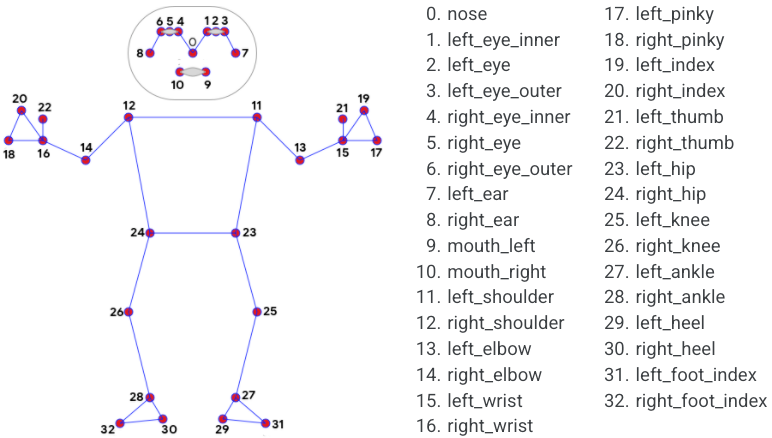
\includegraphics[width=0.8\textwidth]{images/mediapipeNODES.png}
    \caption{MediaPipe Skeleton-Node-Ausgabe mit Koordinaten und Confidence-Werten}
    \label{fig:mediapipe_nodes}
\end{figure}

\begin{figure}[H]
    \centering
    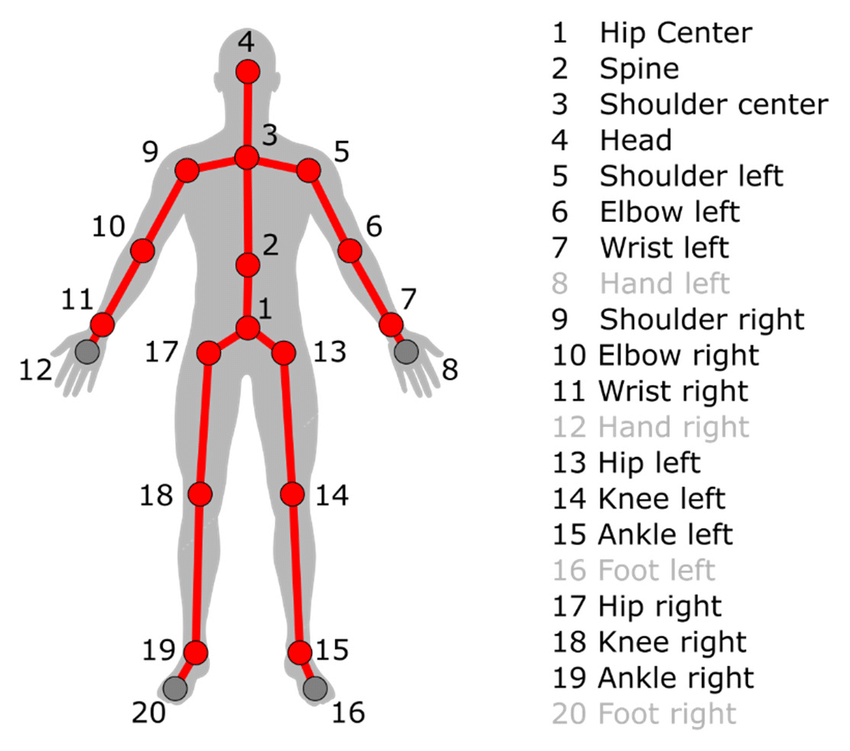
\includegraphics[width=0.8\textwidth]{images/kinect_nodes.png}
    \caption{Kinect V2 Skeleton-Visualisierung mit Node-Nummerierung}
    \label{fig:kinect_nodes}
\end{figure}

\subsubsection{Komparative Tracking-Evaluation}

\textbf{Testsetup:}
Simultanes MediaPipe- und Kinect-Tracking über gemeinsame RGB-Kamera der Kinect V2.

\textbf{Testumgebung:}
\begin{itemize}
    \item \textbf{TouchDesigner-Interface:} Siehe Abbildung \ref{fig:testing_interface}
    \item \textbf{Repository:} \texttt{Testing\_KinectVsMediapipe.toe}
    \item \textbf{Demonstration:} \url{YOUTUBE_LINK_HIER_EINFUEGEN}
\end{itemize}

\begin{figure}[H]
    \centering
    % \includegraphics[width=0.9\textwidth]{images/KINECTMediaPipe_Testing.png}
    \caption{TouchDesigner-Interface für komparative Tracking-Tests}
    \label{fig:testing_interface}
\end{figure}

\textbf{Evaluationsergebnisse:}
MediaPipe demonstriert signifikant verbesserte Robustheit bei partieller Okklusion. Das ML-Modell generiert höhere Confidence-Werte für nicht-sichtbare Körperregionen (z.B. bei Rotationsbewegungen) im Vergleich zur nativen Kinect-Hardware-Implementierung.

\textbf{Technische Implikationen:}
\begin{itemize}
    \item MediaPipe eignet sich als primäres Tracking-System für komplexe Choreographien
    \item Kinect V2 fungiert als Backup-System und Tiefendatenquelle
    \item Hybride Implementierung maximiert Tracking-Reliabilität
\end{itemize}